\documentclass[11pt,a4paper]{scrartcl}
%\documentclass[11pt,a4paper]{article}
\usepackage{xcolor}
\usepackage[affil-it]{authblk}
\usepackage{geometry}
\usepackage{url}
\usepackage{natbib}
%\usepackage{libertine}
\usepackage{pgfgantt}
\usepackage{graphicx}
\usepackage{amsmath}
\usepackage{amssymb}
\usepackage{booktabs}
\usepackage{hyperref}
% The title of your topic should be succinct.
% Less than 15 words is the rule of thumb.
\title{

\includegraphics[height=5cm,width=0.8\textwidth]{westernsydney_logo.PNG}\\
Project Report}
\author{
	Martin Sekuloski\\
	Amani Sarraj\\
	Forrest Hogan}
\affil{Assignment 1 for 301034 Predictive Modelling}


\affil{School of Computer, Data and Mathematical Sciences, \\ Western Sydney University}

\date{Spring, 2021}


\begin{document}

\maketitle

% This proposal document is the starting point and will gradually evolve
% into the final progress report for this unit and the final report for
% the subsequent unit.

\newpage

\section*{Declaration}

By including this statement, we the authors of this work, verify that:
\begin{itemize}
	\item We hold a copy of this assignment that we can produce if the original is lost or damaged.
	\item We hereby certify that no part of this assignment/product has been copied from any other student’s work or from any other source except where due acknowledgement is made in the assignment.
	\item No part of this assignment/product has been written/produced for us by another person except where such collaboration has been authorised by the subject lecturer/tutor concerned.
	\item We are aware that this work may be reproduced and submitted to plagiarism detection software programs for the purpose of detecting possible plagiarism (which may retain a copy on its database for future plagiarism checking).
	\item We hereby certify that we have read and understand what the School of Computer, Data and Mathematical Sciences defines as minor and substantial breaches of misconduct as outlined in the learning guide for this unit.
\end{itemize}


\newpage

\section{Question 1}
Code can be located at :  \href{https://github.com/MS19393924/Assignment-1-Group-9/blob/8bc1cdcf89aecd67f765e19b0435afb995805ea6/Amani_18831506.py}{\textcolor{blue}{Python File Q1}} \\
Save the dataset in the library, import in jupyter as csv file. view the dataset and check the information of it.\\

This dataset contains 12 variables, one variable is ordinal and the rest are numerical.\\

When creating the train and test datasets correctly, 80\% of the dataset goes into the training set and 20\% into testing set. Create a linear regression to predict the training set and get the R square. Calculate the accuracy of regression model of the testing and training set. Lastly calculate the RMSE.\\

Accuracy comes out to 68.77 \%. That means our data classifier is doing a good job.\\

Check R square to know how well our model fits. R square is 68.8 \% almost 70\% that means is a good model. Also, we have RMSE is 59.97\%

\newpage
\section{Question2}
	Create a logistic regression model to predict the quality of each wine sample.\\
Code can be located at :  \href{https://github.com/MS19393924/Assignment-1-Group-9/blob/a2b6a9d1d7f083a31166de573c10290efd0e8029/Forrest/QuestionTwoV2.py}{\textcolor{blue}{Python File Q2}} \\
To pre-process the data I trimmed off the headers and ran a check for any nan and NA values. None were found. After this I search the quality column to find the range and the clustering of the data. I also split the data into 80\% training and 20\% test.
After pre-processing the data I figured that an alternative to using just numpy would be to use pandas as pandas offers a great deal of options with its data frames over numpy’s arrays. I also figured that it would be useful to match single x values of data with y outputs to see the strength of their relationships.\\
I created two classification models one binary and one multi-class. In producing the binary model I treated any value below 5 to be 0 and any over to be 1 and used the liblinear logistic regression. The binary model produced an accuracy of 74\%.
The difference between prediction misclassification from 1 and 0 were negligible. \\
For the multi-class model I split the data by 3.33... so that I had 3 classes. The accuracy of the model was 86\%, However I would like to note that the majority of the data sat in the middle of the dataset and gave little to no information to the lower end of the data set and similarly but not as sever to the higher end of
the spectrum. This is shown in the figure 'Frequency of numbers' where the vast majority of y outputs hover around 5 and 6.\\
To overcome this issue in the future it would be better to use a range the numbers from the 4 to 7 and split the classifications to four values apposed to 3.


\begin{figure}
	\centering
	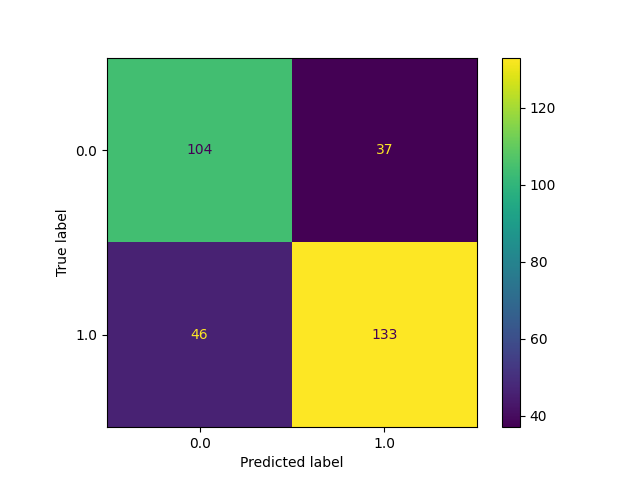
\includegraphics[width=0.95\textwidth]{conMatBinary.png}
	\caption{Binary}
	\label{fig:logo}
\end{figure}
\begin{figure}
	\centering
	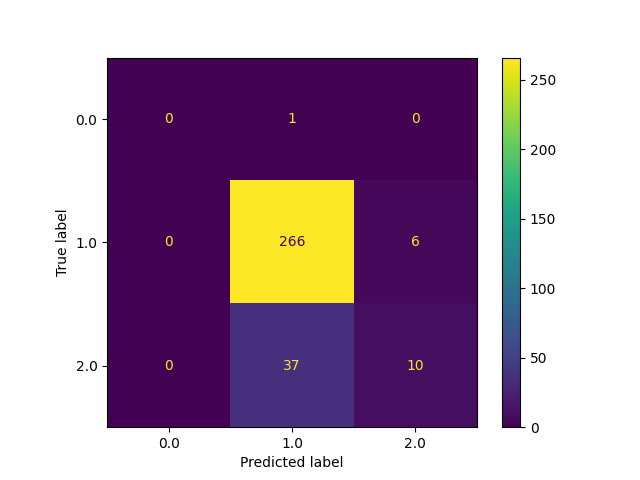
\includegraphics[width=0.95\textwidth]{conMatMulti.png}
	\caption{Multi-Class}
	\label{fig:logo}
\end{figure}	 
\begin{figure}
	\centering
	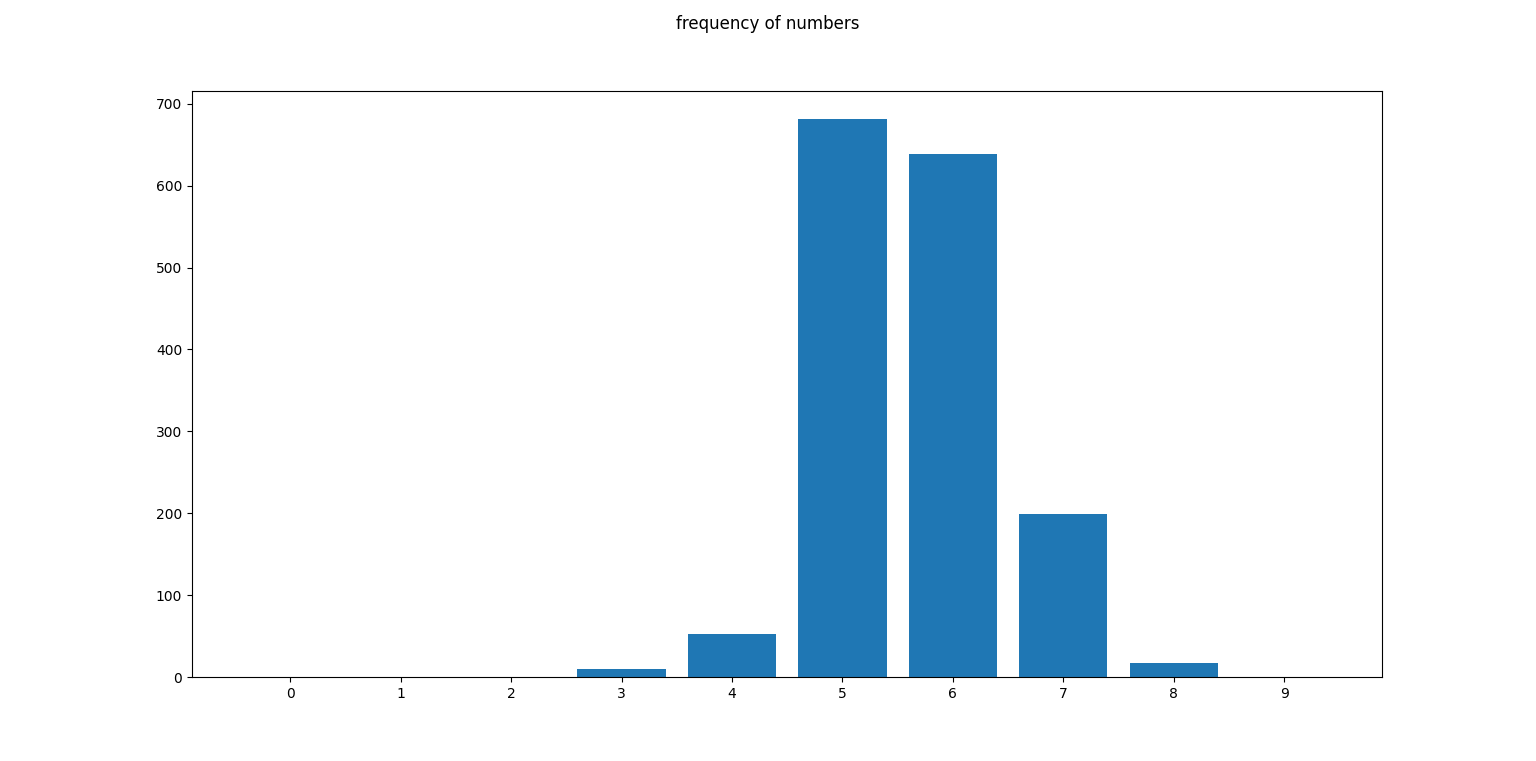
\includegraphics[width=0.95\textwidth]{freqNum.png}
	\caption{Numbers}
	\label{fig:logo}
\end{figure}



\newpage
\section{Question3}
Code can be located at :  \href{https://github.com/MS19393924/Assignment-1-Group-9/blob/8bc1cdcf89aecd67f765e19b0435afb995805ea6/Question3}{\textcolor{blue}{Python File Q3}} \\
Write a brief description of your steps to create your model, including but not limited to the following:\\
- What is the accuracy of your model on the training and test data?\\
- How did you tune the hyperparameter of your model? \\
- Compare this model with the linear regression model in Question 1, did you achieve improvement in your result? \\  
What’s the difference between the two models?\\
Ridge regression being a regularised technique for linear regression. Through the method of L2 regularisation. It works in the sense that a user expects a subset of true coefficients to be small or zero. Creating the model was initially done through importing the dataset through numpy. Once the csv file was imported the X and y variable were defined along with training and testing data sets. The ridge and gridSearch functions were used to then print out the regression model. \\
How did you tune the hyperparameter of your model?\\
The hyperparameter was tuned through the creation of grid searches which compares and chooses the most appropriate alpha value of the dataset.
Compare this model with the linear regression model in Question 1, did you achieve improvement in your result?  \\
-What’s the difference between the two models? \\ 
After comparing both linear and ridge regressions. Both models were working but the Linear Regression proved to be more accurate. Linear regression establishes a connection between x and y variables where as ridge regression is more so a strategy used when data is highly correlated with its x variables.




\end{document}

%%% Local Variables:
%%% mode: latex
%%% TeX-master: t
%%% End:
